\documentclass[12pt,a4paper]{extarticle}
\usepackage[utf8]{inputenc}
\usepackage[T5]{fontenc}
\usepackage{geometry}
\geometry{a4paper, left=1.5cm, right=1cm, top=1.5cm, bottom=1.5cm, headheight=20pt, headsep=15pt, footskip=28pt}
\usepackage{enumitem}
\usepackage{amsmath}
\usepackage{amssymb}
\usepackage{diagbox}
\usepackage{colortbl} % Sửa lỗi \arrayrulecolor
\usepackage{array}    % Hỗ trợ định dạng cột m{2cm}
\usepackage[most]{tcolorbox}
\newcommand{\khongxacdinh}{\text{KXĐ}}
\newcommand{\blackbox}[1]{\texorpdfstring{\fcolorbox{black}{black}{\textcolor{white}{#1}}}{#1}}
\usepackage{tikz}
\definecolor{bookblue}{RGB}{58,90,172}
\definecolor{book}{RGB}{58,90,172}
\definecolor{myblue}{RGB}{200,40,40}
\newcommand{\bluecheck}{\textcolor{myblue}{\checkmark}}
\newtcolorbox{formulaBox}{colback=gray!5,colframe=bookblue,boxrule=0.8pt,arc=2mm}
\newtcolorbox{notebox}{colback=blue!3,colframe=myblue,boxrule=0.8pt,arc=2mm}
\usetikzlibrary{patterns, patterns.meta} % Thêm patterns.meta vào đây
% Gọi package nằm trong thư mục con template
\usepackage{../template/mngocbox}

\begin{document}

% Sử dụng ngoặc vuông [...] để thay đổi linh hoạt các thông số
\makeheadbox[headerright={Chương 5},chude={Bài 1},tieude={Phương trình mặt phẳng},dinhdang={Hình học},lop={12 },gv={Nguyễn Lê Minh Ngọc}]
\vspace{2em}



\section*{\color{myblue}{I. Vectơ pháp tuyến, cặp vectơ chỉ phương của mặt phẳng}}
\subsection*{\color{myblue}{1. Vectơ pháp tuyến}}
\begin{tcolorbox}[colback=lightblue, colframe=myblue, arc=2mm]
Cho mặt phẳng $(P)$. Nếu vectơ $\vec{n} \neq \vec{0}$ và có giá vuông góc với mặt phẳng $(P)$ thì $\vec{n}$ được gọi là \textit{vectơ pháp tuyến} của mặt phẳng $(P)$.
\end{tcolorbox}
\noindent $\star$ \textbf{Nhận xét:} Nếu $\vec{n}$ là vectơ pháp tuyến của một mặt phẳng thì $k\vec{n}$ ($k \neq 0$) cũng là vectơ pháp tuyến của mặt phẳng đó.
\subsection*{\color{myblue}{2. Cặp vectơ chỉ phương}}
\begin{tcolorbox}[colback=lightblue, colframe=myblue, arc=2mm]
Cho mặt phẳng $(P)$. Hai vectơ không cùng phương có giá song song hoặc nằm trong mặt phẳng $(P)$ được gọi là \textit{cặp vectơ chỉ phương} của mặt phẳng $(P)$.
\end{tcolorbox}
\subsection*{\color{myblue}{3. Xác định vectơ pháp tuyến khi biết cặp vectơ chỉ phương}}
\begin{tcolorbox}[colback=lightblue, colframe=myblue, arc=2mm]
Nếu hai vectơ $\vec{a} = (a_1; a_2; a_3), \vec{b} = (b_1; b_2; b_3)$ là cặp vectơ chỉ phương của mặt phẳng $(P)$ thì:
\[
\vec{n} = [\vec{a}, \vec{b}] = \left( 
\begin{vmatrix} a_2 & a_3 \\ b_2 & b_3 \end{vmatrix}; 
\begin{vmatrix} a_3 & a_1 \\ b_3 & b_1 \end{vmatrix}; 
\begin{vmatrix} a_1 & a_2 \\ b_1 & b_2 \end{vmatrix} 
\right)
\]
là một vectơ pháp tuyến của mặt phẳng $(P)$.
\end{tcolorbox}
\vspace{0.4cm}
\section*{\color{myblue}{II. Phương trình tổng quát của mặt phẳng}}
\begin{tcolorbox}[colback=lightblue, colframe=myblue, arc=2mm]
Phương trình $Ax + By + Cz + D = 0$ ($A, B, C$ không đồng thời bằng $0$) là \textit{phương trình tổng quát} của mặt phẳng. Hệ số $D$ gọi là \textit{hệ số tự do} của phương trình tổng quát.
\end{tcolorbox}
\noindent $\star$ \textbf{Nhận xét:} Nếu mặt phẳng có phương trình tổng quát là $Ax + By + Cz + D = 0$ thì nó có một vectơ pháp tuyến là $\vec{n} = (A; B; C)$.
\vspace{0.4cm}
\section*{\color{myblue}{III. Lập phương trình tổng quát của mặt phẳng biết một số điều kiện}}
\subsection*{\color{myblue}{1. Đi qua một điểm và biết số vectơ pháp tuyến}}
\begin{tcolorbox}[colback=lightblue, colframe=myblue, arc=2mm]
Mặt phẳng $(P)$ đi qua điểm $I(x_0; y_0; z_0)$ và nhận $\vec{n} = (A; B; C)$ làm vectơ pháp tuyến có phương trình tổng quát là $Ax + By + Cz + D = 0$ với $D = -Ax_0 - By_0 - Cz_0$.
\end{tcolorbox}
\noindent $\star$ \textbf{Chú ý:} Phương trình mặt phẳng $(P)$ đi qua điểm $I(x_0; y_0; z_0)$ và nhận $\vec{n} = (A; B; C)$ làm vectơ pháp tuyến có dạng:
\[
A(x - x_0) + B(y - y_0) + C(z - z_0) = 0.
\]
\subsection*{\color{myblue}{2. Đi qua một điểm và biết cặp vectơ chỉ phương}}
Để lập phương trình mặt phẳng $(P)$ đi qua điểm $I(x_0; y_0; z_0)$ có cặp vectơ chỉ phương là $\vec{u}, \vec{v}$ ta làm như sau:
\begin{itemize}
    \item[\textbf{•}] \textbf{Bước 1:} Tìm $\vec{n} = [\vec{u}, \vec{v}]$.
    \item[\textbf{•}] \textbf{Bước 2:} Lập phương trình mặt phẳng $(P)$ đi qua điểm $I(x_0; y_0; z_0)$ nhận $\vec{n}$ làm vectơ pháp tuyến.
\end{itemize}

\subsection*{\color{myblue}{3. Lập phương trình tổng quát của mặt phẳng đi qua ba điểm không thẳng hàng}}
Để lập phương trình mặt phẳng $(P)$ đi qua ba điểm $H(a_1; b_1; c_1), I(a_2; b_2; c_2), K(a_3; b_3; c_3)$ không thẳng hàng, ta có thể làm như sau:
\begin{itemize}
    \item[\textbf{•}] \textbf{Bước 1:} Tìm cặp vectơ chỉ phương của mặt phẳng $(P)$ là:
    \[
    \vec{HI} = (a_2 - a_1; b_2 - b_1; c_2 - c_1), \quad \vec{HK} = (a_3 - a_1; b_3 - b_1; c_3 - c_1)
    \]
    \item[\textbf{•}] \textbf{Bước 2:} Tìm $\vec{n} = [\vec{HI}, \vec{HK}]$.
    \item[\textbf{•}] \textbf{Bước 3:} Lập phương trình mặt phẳng $(P)$ đi qua điểm $H(a_1; b_1; c_1)$ nhận $\vec{n}$ làm vectơ pháp tuyến.
\end{itemize}
\vspace{0.2cm}
\begin{tcolorbox}[colback=lightblue, colframe=myblue, arc=2mm]
\noindent $\star$ \textbf{Chú ý:} Mặt phẳng đi qua ba điểm $A(a; 0; 0), B(0; b; 0), C(0; 0; c)$ với $abc \neq 0$ có phương trình là:
\[
\frac{x}{a} + \frac{y}{b} + \frac{z}{c} = 1
\]
Phương trình đó còn được gọi là \textbf{phương trình mặt phẳng theo đoạn chắn}.
\end{tcolorbox}
\vspace{0.3cm}
% ================= HÌNH VẼ TIKZ MẶT PHẲNG ĐOẠN CHẮN =================
\begin{center}
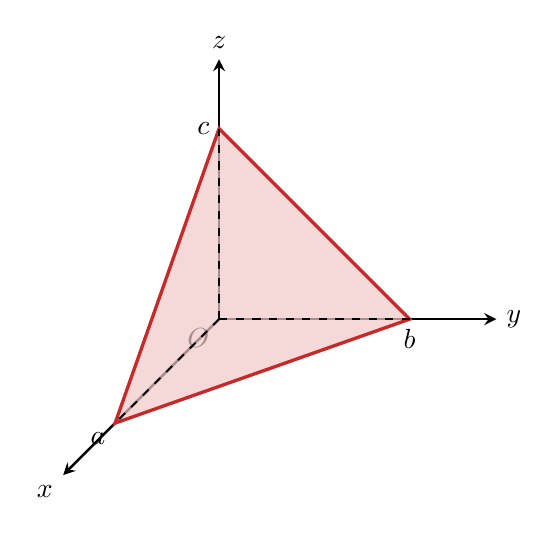
\begin{tikzpicture}[scale=1.1, >=stealth]
  % Các trục tọa độ
  \draw[->, line width=0.9pt] (0,0) -- (-1.8,-1.8) node[below left] {$x$};
  \draw[->, line width=0.9pt] (0,0) -- (3.2,0) node[right] {$y$};
  \draw[->, line width=0.9pt] (0,0) -- (0,3.0) node[above] {$z$};
  \node[below left] at (0,0) {$O$};
  % Các giao điểm a, b, c
  \coordinate (A) at (-1.2,-1.2);
  \coordinate (B) at (2.2,0);
  \coordinate (C) at (0,2.2);
  % Tô màu tam giác đoạn chắn
  \fill[myblue!25, opacity=0.7] (A) -- (B) -- (C) -- cycle;
  \draw[line width=1.2pt, myblue] (A) -- (B) -- (C) -- cycle;
  % Đường nét đứt bên trong
  \draw[dashed, line width=0.7pt] (0,0) -- (A);
  \draw[dashed, line width=0.7pt] (0,0) -- (B);
  \draw[dashed, line width=0.7pt] (0,0) -- (C);
  % Tên nhãn các điểm giao
  \node[below left] at (A) {$a$};
  \node[below] at (B) {$b$};
  \node[left] at (C) {$c$};
\end{tikzpicture}
\end{center}
% ======================================================================
\vspace{0.4cm}
\section*{\color{myblue}{IV. Điều kiện song song, vuông góc của hai mặt phẳng}}
\subsection*{\color{myblue}{1. Điều kiện song song của hai mặt phẳng}}
\begin{tcolorbox}[colback=lightblue, colframe=myblue, arc=2mm]
Cho mặt phẳng $(P_1)$ có phương trình $A_1x + B_1y + C_1z + D_1 = 0$ và mặt phẳng $(P_2)$ có phương trình $A_2x + B_2y + C_2z + D_2 = 0$.
\vspace{0.2cm}
Gọi $\vec{n}_1 = (A_1; B_1; C_1), \vec{n}_2 = (A_2; B_2; C_2)$ lần lượt là vectơ pháp tuyến của $(P_1)$ và $(P_2)$. Khi đó:
\[
(P_1) \parallel (P_2) \iff \text{tồn tại số thực } k \neq 0 \text{ sao cho } 
\begin{cases} 
\vec{n}_1 = k\vec{n}_2 \\ 
D_1 \neq kD_2 
\end{cases}
\]
\end{tcolorbox}
\subsection*{\color{myblue}{2. Điều kiện vuông góc của hai mặt phẳng}}
\begin{tcolorbox}[colback=lightblue, colframe=myblue, arc=2mm]
Cho mặt phẳng $(P_1)$ có phương trình $A_1x + B_1y + C_1z + D_1 = 0$ và mặt phẳng $(P_2)$ có phương trình $A_2x + B_2y + C_2z + D_2 = 0$. Khi đó:
\[
(P_1) \perp (P_2) \iff A_1A_2 + B_1B_2 + C_1C_2 = 0
\]
\end{tcolorbox}
\vspace{0.4cm}
\section*{\color{myblue}{V. Khoảng cách từ một điểm đến một mặt phẳng}}
\begin{tcolorbox}[colback=lightblue, colframe=myblue, arc=2mm]
Khoảng cách từ điểm $M_0(x_0; y_0; z_0)$ đến mặt phẳng $(P): Ax + By + Cz + D = 0$ ($A^2 + B^2 + C^2 > 0$) được tính theo công thức:
\[
d(M_0, (P)) = \frac{|Ax_0 + By_0 + Cz_0 + D|}{\sqrt{A^2 + B^2 + C^2}}
\]
\end{tcolorbox}


\end{document}